\documentclass[12pt]{article}
\usepackage{graphicx}
\usepackage{amsmath}
\usepackage{mathtools}
\usepackage{gensymb}

\newcommand{\mydet}[1]{\ensuremath{\begin{vmatrix}#1\end{vmatrix}}}
\providecommand{\brak}[1]{\ensuremath{\left(#1\right)}}
\providecommand{\norm}[1]{\left\lVert#1\right\rVert}
\newcommand{\solution}{\noindent \textbf{Solution: }}
\newcommand{\myvec}[1]{\ensuremath{\begin{pmatrix}#1\end{pmatrix}}}
\let\vec\mathbf

\begin{document}
\begin{center}
\textbf\large{CHAPTER-7 \\ COORDINATE GEOMETRY}
\end{center}
\section*{Excercise 7.1}

Q1. Find the distance between the following pairs of points :
\begin{enumerate}
	\item $\brak{2,3}, \brak{4,1}$ 
	\item $\brak{-5,7}, \brak{-1,3}$
	\item $\brak{a,b}, \brak{-a,-b}$
\end{enumerate}
\solution
\begin{enumerate}
\item The coordinates are given as
	\begin{align}
	\vec{A} = \myvec{
		2\\
		3\\
		},
	\vec{B} = \myvec{
		4\\
		1\\
		}
	\end{align}
	\begin{align}
		\vec{A} - \vec{B} = \myvec{2\\3} - \myvec{4\\1} = \myvec{-2\\2}		
	\end{align}
	
	
	
	\begin{align}
		(\vec{A}-\vec{B})^\top (\vec{A}-\vec{B}) = \myvec{-2&2} \myvec{-2\\2} = 4+4 = 8
	\end{align}
	
	\begin{align}
	d={\norm{\vec{A}-\vec{B}}}=\sqrt{\brak{\vec{A} -\vec{B}}^{\top}\brak{\vec{A} -\vec{B}}}
	\end{align}

\begin{align}
d=\sqrt{\brak{\vec{A} -\vec{B}}^{\top}\brak{\vec{A} -\vec{B}}}
 &=\sqrt{8}=2\sqrt{2}=2.828
\end{align}	
	
	Hence the distance between the two points $AB$ is 2.828  shown in Figure:\ref{fig:Fig}


\item The coordinates are given as
	\begin{align}
	\vec{C} = \myvec{
		-5\\
		7\\
		},
	\vec{D} = \myvec{
		-1\\
		3\\
		}
	\end{align}
	\begin{align}
		\vec{C} - \vec{D} = \myvec{-5\\7} - \myvec{-1\\3} = \myvec{-4\\4}		
	\end{align}
	
	
	
	\begin{align}
		(\vec{C}-\vec{D})^\top (\vec{C}-\vec{D}) = \myvec{-4&4} \myvec{-4\\4} = 16+16 = 32
	\end{align}
	
	\begin{align}
		d=\norm{\vec{C}-\vec{D}}=\sqrt{\brak{\vec{C} -\vec{D}}^{\top}\brak{\vec{C} -\vec{D}}}
	\end{align}

\begin{align}
d=\sqrt{\brak{\vec{C} -\vec{D}}^{\top}\brak{\vec{C} -\vec{D}}}
 &=\sqrt{32}=4\sqrt{2}=5.656
\end{align}	
	Hence the distance between the two points $CD$ is 5.656 shown in Figure:\ref{fig:Fig}
	

	
\item The coordinates are given as
	\begin{align}
	\vec{E} = \myvec{
		a\\
		b\\
		},
	\vec{F} = \myvec{
		-a\\
		-b\\
		}
	\end{align}
	\begin{align}
		\vec{E} - \vec{F} = \myvec{a\\b} - \myvec{-a\\-b} = \myvec{2a\\2b}		
	\end{align}
	
	
	
	\begin{align}
		(\vec{E}-\vec{F})^\top (\vec{E}-\vec{F}) = \myvec{2a&2b} \myvec{2a\\2b} = 4a^2+4b^2 
	\end{align}
	
	\begin{align}
		d=\norm{\vec{E}-\vec{F}}=\sqrt{\brak{\vec{E} -\vec{F}}^{\top}\brak{\vec{E} -\vec{F}}}
	\end{align}

\begin{align}
d=\sqrt{\brak{\vec{E} -\vec{F}}^{\top}\brak{\vec{E} -\vec{F}}}
 &=\sqrt{4a^2+4b^2 }=2\sqrt{a^2+b^2}
\end{align}	
 Suppose, if a=1,b=2 , then d = $2\sqrt{1^2+2^2}$ = 4.472\\
	\\Hence the distance between the two points $EF$ is $2\sqrt{a^2+b^2}$ = 4.472 shown in Figure:\ref{fig:Fig}

\begin{figure}[!h]
	\begin{center} 
	    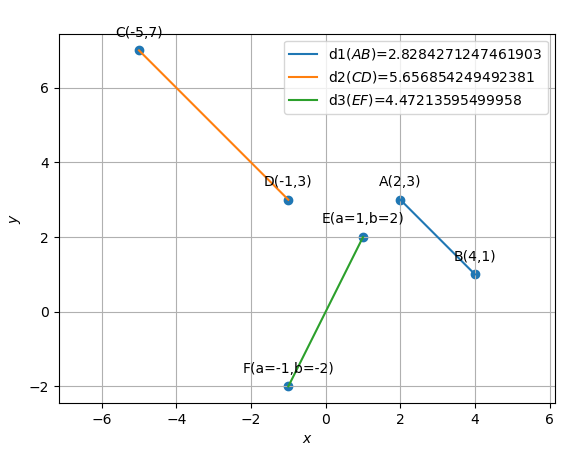
\includegraphics[width=\columnwidth]{./figs/graph.png}
	\end{center}
\caption{}
\label{fig:Fig}
\end{figure}
\end{enumerate}
\end{document}